\section{Axial Loading}

\subsection{\blue{Notation and Convention}}

\begin{figure*}[!h]
\centering
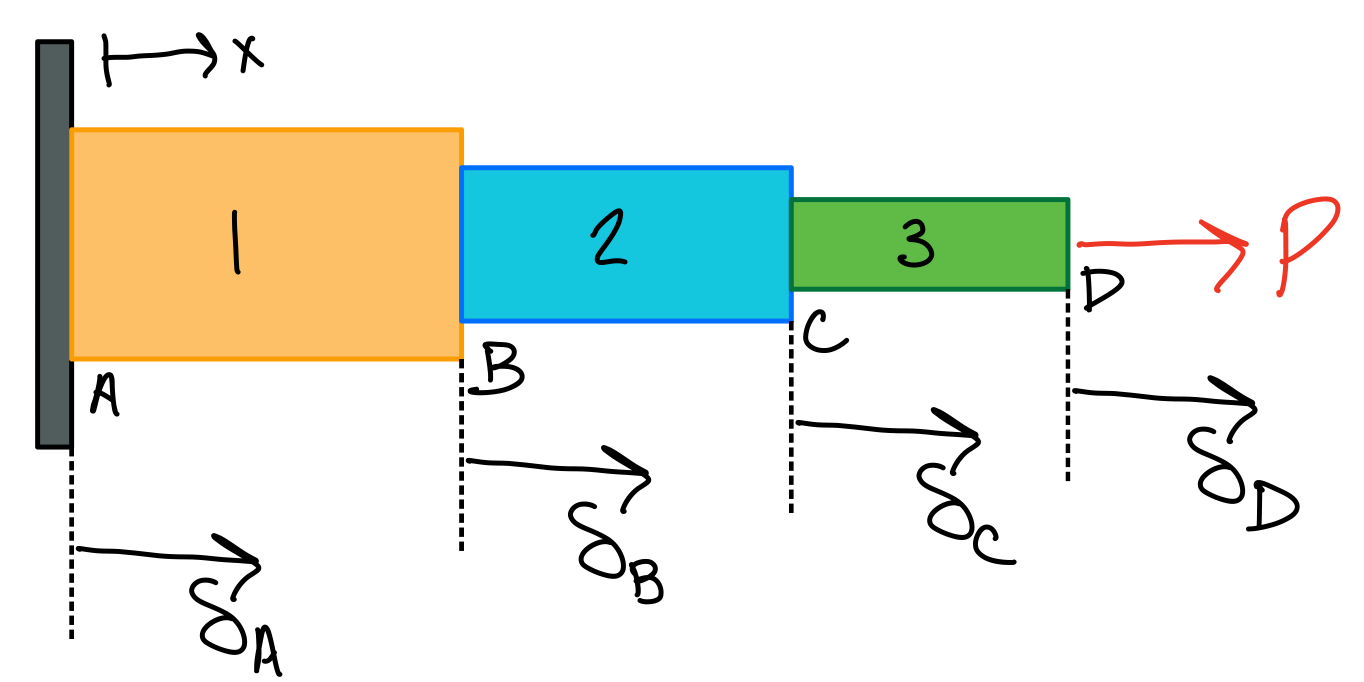
\includegraphics[angle=0, width=3in]{Axial Loading-Figures/Notation.png}
\vspace{-2mm}
\caption{\small \blue{Taken from TAM251 Lecture Notes - L4S4}}
\vspace{-3mm}
\label{Fig:NotationExample}
\end{figure*}
\blue{
\begin{itemize}
    \item \textbf{Displacement of points in space:} the movement of a point relative to its initial position in space (ex; $\delta_B$)
    \item \textbf{Change in length of a segment:} the relative displacement of a point with respect to another point (ex; $\delta_{B/A} = \delta_B - \delta_A = \delta_1$). This can be written multiple ways:
    \[\delta_{AD} \equiv \delta_{DA} \equiv \delta_{A/D} \equiv \delta_{D/A}\]
\end{itemize}
\textbf{Sign Conventions \cyan{BSM: for the forces, it would be wise to note the convention applies specifically to *internal* force in a bar.}}
\begin{itemize}
    \item $F>0$: tension
    \item $F<0$: compression
    \item $\delta>0$: elongation
    \item $\delta<0$: contraction
\end{itemize}
}

\subsection{Saint-Venant's Principle: slender beam case}

Stress analysis very near to the point of application of load $P$. \textbf{Saint-Venant's principle:} the stress and strain produced at points in a body \textit{sufficiently removed}* from the region of external load application will be the same as the stress and strain produced by any other applied external loading that has the same statically equivalent resultant and is applied to the body within the same region. 

\noindent *farther than the widest dimension of the cross section

\cyan{BSM: a figure would go a long way to clarifying this point, Hibbeler textbook probably has something to use for inspiration.}

\subsection{Force-Deformation Relation}

\[\delta = \frac{PL}{EA}\]

\noindent Axial Flexibility: \[\delta = fP   =>   f = \frac{L}{EA}\]

\noindent Axial Stiffness: \[P = k\delta   =>   k = \frac{EA}{L}\]

\noindent \textbf{*Expandable Derivation*}

\[P = \sigma A\]
\[\sigma = E\varepsilon\]
\[\varepsilon = \delta / L\]
\[=>   P = E\frac{\delta}{L}A\]
\noindent \textbf{**End Derivation**}

\subsection{\blue{Axially Varying Properties}} 
For non-uniform load, material property and cross-section area:

 \[\delta = \int_0^L\frac{F(x)}{E(x)A(x)}dx\]

\noindent Assume variations with $x$ are "mild" (on length scale longer than cross-sectional length scales)

\blue{
\noindent \textbf{*Expandable Derivation*}
\[\sigma = E\varepsilon\]
\[\frac{F(x)}{A(x)} = E(x)\varepsilon(x)\]
\[\frac{F(x)}{A(x)} = E(x)\frac{d\delta(x)}{dx}\]
\[d\delta = \frac{F(x)}{E(x)A(x)}dx\]
}
\noindent \blue{\textbf{**End Derivation**}}

\subsection{Principle of Superposition }

Superposition: If the displacements are (1) small and (2) linearly related to the force components acting, the displacements caused by the components can be added up:

\[\delta = \sum_i \delta_i = \sum_i \frac{F_i L_i}{E_i A_i}\]

\subsection{General Solving Procedure}

\begin{enumerate}
    \item Draw a FBD
    \item Equilibrium equations: force balance and moment balance
    \item Constitutive equations: stress-strain or force-displacement relations
    \item Compatibility equations: geometric constraints
\end{enumerate}

\subsection{\blue{Statically Determinate Problems}}

\begin{figure*}[!h]
\centering
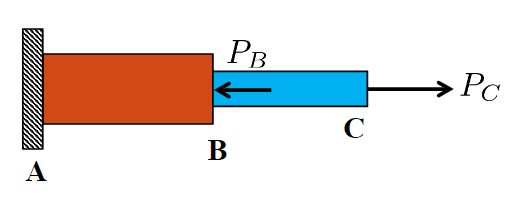
\includegraphics[angle=0, width=3in]{Axial Loading-Figures/StaticallyDeterminate.png}
\vspace{-2mm}
\caption{\small \blue{Taken from TAM251 Lecture Notes - L4S9}}
\vspace{-3mm}
\label{Fig:Determinate}
\end{figure*}

\noindent \blue{All internal forces can be obtained from equilibrium analysis only}

\subsection{Statically Indeterminate Problems}

\begin{figure*}[!h]
\centering
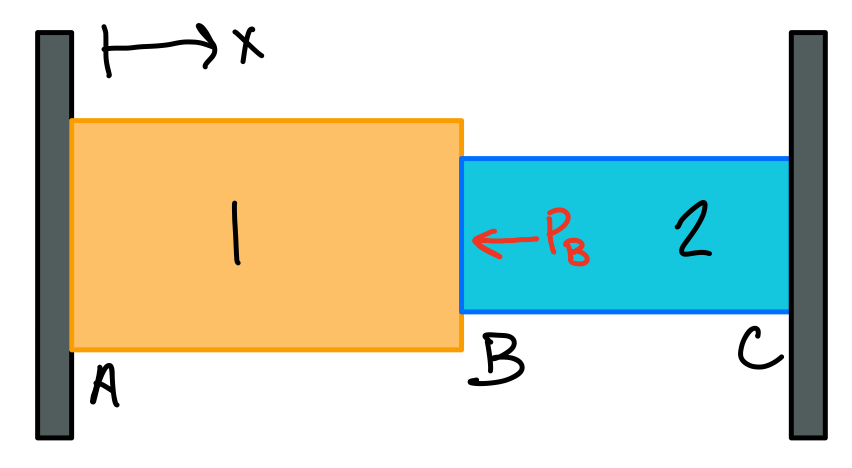
\includegraphics[angle=0, width=3in]{Axial Loading-Figures/StaticallyIndeterminate.png}
\vspace{-2mm}
\caption{\small \blue{Taken from TAM251 Lecture Notes - L4S10}}
\vspace{-3mm}
\label{Fig:Indeterminate}
\end{figure*}

\noindent Equilibrium does not determine all internal forces.

\subsubsection{\blue{Thermal Effects: Temperature Changes}}

\blue{
\textbf{Notation}
\begin{itemize}
    \item $\Delta T > 0, \sigma < 0$: Compression
    \item $\Delta T < 0, \sigma > 0$: tension
\end{itemize}
}


\noindent \blue{$\delta_T$, $\varepsilon_T$ present in addition to elastic $\delta_E$, $\varepsilon_E$ (from internal forces). Superposition (small strains):
\[\varepsilon_{tot} = \varepsilon_{E} + \varepsilon_{T}\]
 \[\delta_{tot} = \delta_{E} + \delta_{T}\]
}

\begin{figure*}[!h]
\centering
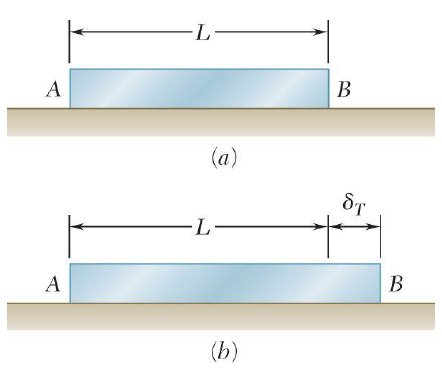
\includegraphics[angle=0, width=3in]{Axial Loading-Figures/Temperature_NoLoad.png}
\vspace{-2mm}
\caption{\small \blue{Taken from TAM251 Lecture Notes - L4S17}}
\vspace{-3mm}
\label{Fig:TempNoLoad}
\end{figure*}

\noindent A rod rests freely on a smooth horizontal surface. Temperature of the rod is raised by $\Delta T$. Rod elongates by an amount.

\[\delta_{T} = \alpha \Delta T L\]

\noindent Linear coefficient of thermal expansion $\alpha$,  $[\alpha] = \frac{1}{K},\frac{1}{°C},...$. This deformation is associated with an average thermal strain:

\[\varepsilon_{T} = \frac{\delta_T}{L} = \alpha T\]

\begin{figure*}[!h]
\centering
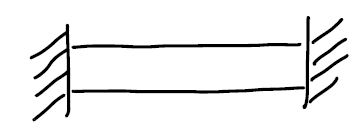
\includegraphics[angle=0, width=2in]{Axial Loading-Figures/Temperature_TwoPlates.png}
\vspace{-2mm}
\caption{\small \blue{Taken from TAM251 Lecture Notes - L4S17}}
\vspace{-3mm}
\label{Fig:TempNoLoad}
\end{figure*}

\noindent Initially, rod of length $L$ is placed between two supports at a distance $L$ from each other. With no internal forces, there is no stress or strain.

\[R_{A} = R_{B} = 0\]
\[R_{A} = F\]
                  
\noindent After raising the temperature, the total elongation of the rod is still zero. The total elongation is given by:

\[\delta = \frac{FL}{EA} + \alpha L \Delta T = 0\]

\noindent The stress in the rod due to change in temperature is given by:
\[\sigma = -\alpha E \Delta T\]

\subsubsection{Misfit Problems}
A misfit problem is one in which there is difference between a design distance and the manufactured length of a material. Some misfits are created intentionally to pre-strain a member. (e.g. spokes in a bicycle wheel or strings in a tennis racket). This type of problem neither modifies the equilibrium equations (1) nor the force-extension relations, (2) but the compatibility equations, (3) need to be modified.

\subsection{Stress Concentration \cyan{BSM: we do not cover this topic in class/hw/exams. It is covered in ME 330 and ME 371.}}

\noindent Highest at lowest cross-sectional area.

Stress concentration factor: \[K = \frac{\sigma_{max}}{\sigma_{avg}}\]

\begin{itemize}
    \item Found experimentally
    \item Solely based on geometry
\end{itemize}

\noindent \textbf{\red{**Reference pages have a broken link image here**}}
